\documentclass{article} \usepackage[margin=1in,headheight=57pt,headsep=0.1in]{geometry}
\usepackage{xcolor}
\usepackage{tikz}
\usepackage{float}
\usepackage{longtable}
\usepackage[framemethod=TikZ]{mdframed}
\usepackage{fancyhdr}
\usepackage[utf8]{inputenc} % Required for inputting international characters
\usepackage[T1]{fontenc} % Output font encoding for international characters
\usepackage{stix} % Use the STIX fonts
\usepackage{hyperref}
\hbadness=99999

% ------------- %
% HEADER/FOOTER %
% ------------- %
\setlength\parindent{0pt}
\setlength\headheight{30pt}
\headsep=0.25in
\lhead{\textbf{tbrpggepp User Manual}}
\rhead{\textbf{12SDD}}


% -------- %
% DOCUMENT %
% -------- %
\begin{document}

% ---------- %
% TITLE PAGE %
% ---------- %
\begin{titlepage} % Suppresses displaying the page number on the title page and the subsequent page counts as page 1

	\raggedleft % Right align the title page

	\rule{1pt}{\textheight} % Vertical line
	\hspace{0.05\textwidth} % Whitespace between the vertical line and title page text
	\parbox[b]{0.75\textwidth}{ % Paragraph box for holding the title page text, adjust the width to move the title page left or right on the page

		{\Huge\bfseries tbrpggepp User Manual}\\[2\baselineskip] % Title
		{\large\textit{Tutorial and Troubleshooting Guide}}\\[4\baselineskip] % Subtitle or further description
		{\Large\textsc{james denovan}} % Author name, lower case for consistent small caps

		\vspace{0.5\textheight} % Whitespace between the title block and the publisher

		{\noindent Kinross Wolarai School}\\[\baselineskip] % Publisher and logo
	}

\end{titlepage}
\thispagestyle{empty}
\tableofcontents
\pagebreak
\pagestyle{fancy}
\section{Introduction}
tbrpggepp (Text-Based Role-Playing Game Graphical Editor Plus Plus) is a graphical desktop program for creating the narratives of branching text-based computer games. The program works on both Linux and Windows systems, and has two requirements: a working installation of \texttt{Python 3.7} and the Python library \texttt{PyQt5}, which you can install by entering the following command in a terminal: \\

\texttt{pip install PyQt5} \\

Within tbrpggepp, you create the game-world that the player character navigates throughout their quest. You write the words that the player sees, the enemies and scenarios they encounter, and how they navigate your world. You can write a game about anything: from exploring ancient dungeons, to escaping derelict space stations. The only limit is your imagination. \\

To run the program, simply double-click the \texttt{mainMenuForm.py} file and Python should do the rest.
\newpage
\section{Using the Program}
\subsection{The Introduction Form}
\begin{figure}[H]
	\centering
	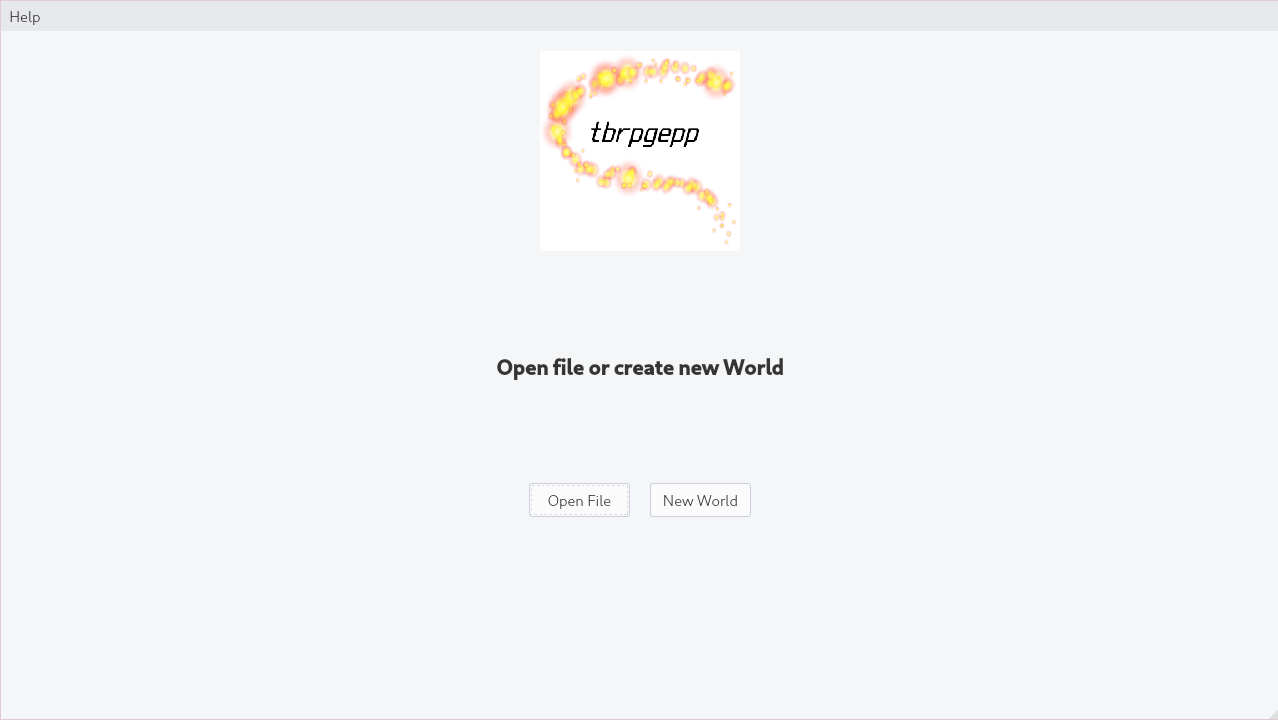
\includegraphics[width=1.0\textwidth]{./introForm.png}
\end{figure}
This is the first form you see when you execute the \texttt{mainMenuForm.py} file. You are presented with two options: open a preexisting file containing a \texttt{tbrpggepp} game world, or create a new one.
\subsubsection{Creating a new game-world}
\begin{figure}[H]
	\centering
	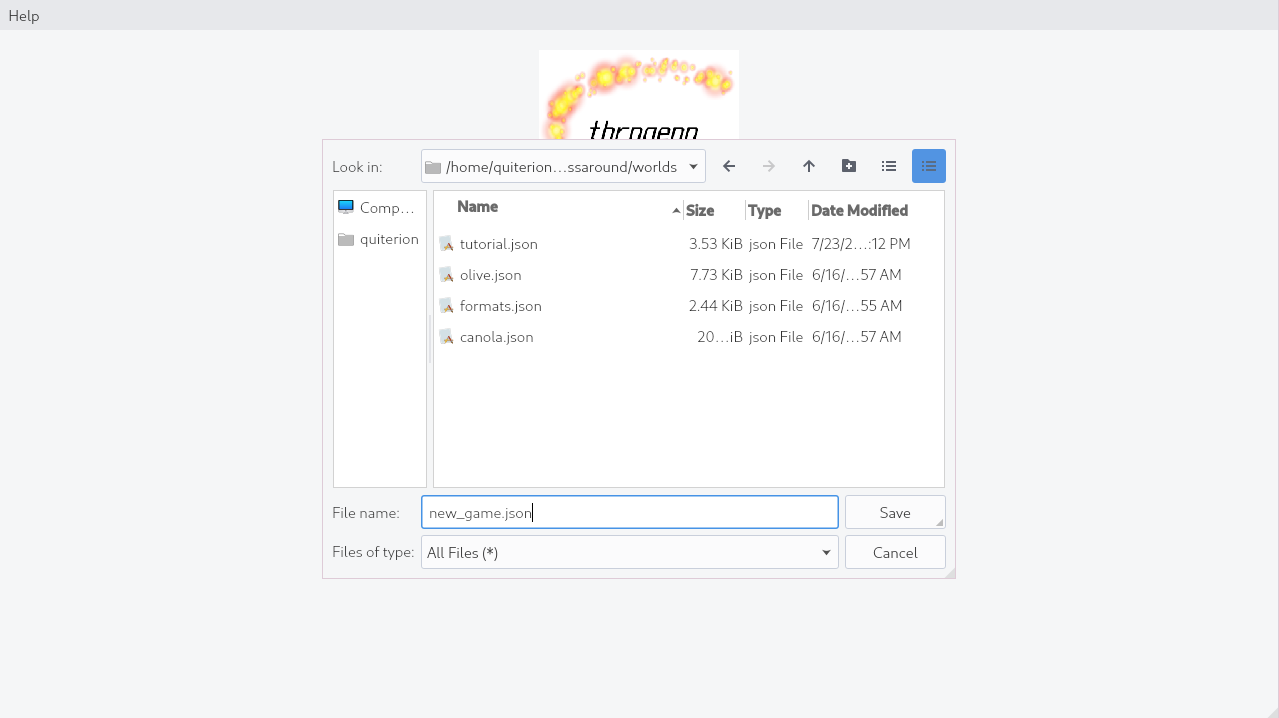
\includegraphics[width=1.0\textwidth]{./introFormWithFileDialog.png}
\end{figure}
Upon clicking "New World", a dialog will appear prompting you to create a new file. You may create this file in any directory you please, but \textbf{note that game-world files must have a "\texttt{.json}" extension.} After creating a file, the Introduction form will close and take you to the Main Menu form.
\subsubsection{Opening a preexisting game-world file}
\begin{figure}[H]
	\centering
	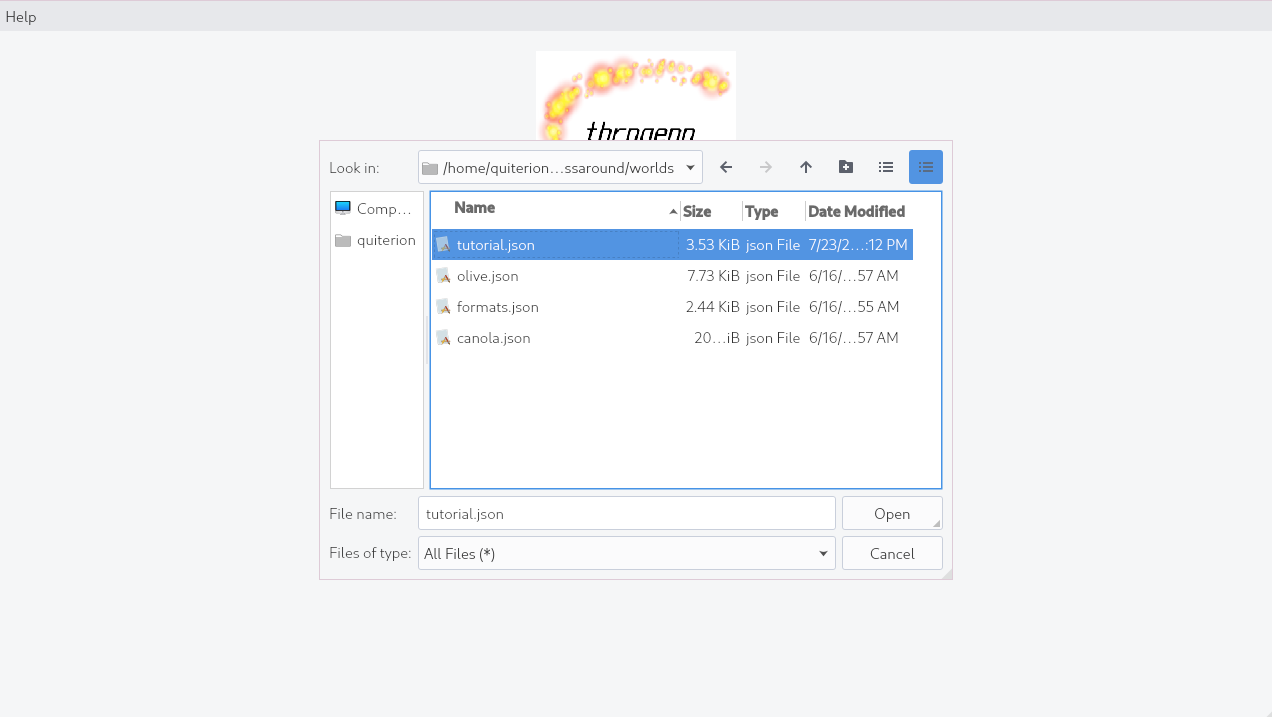
\includegraphics[width=1.0\textwidth]{./introFormWithOpenFileDialog.png}
\end{figure}
Upon clicking "Open File" an identical dialog will appear, this time prompting you to select a preexisting file. \textbf{Note that a valid game-world file must end in a "\texttt{.json}" extension.} After selecting a file, the Introduction form will close and take you to the Main Menu form.
\newpage
\subsection{The Main Menu Form}
\begin{figure}[H]
	\centering
	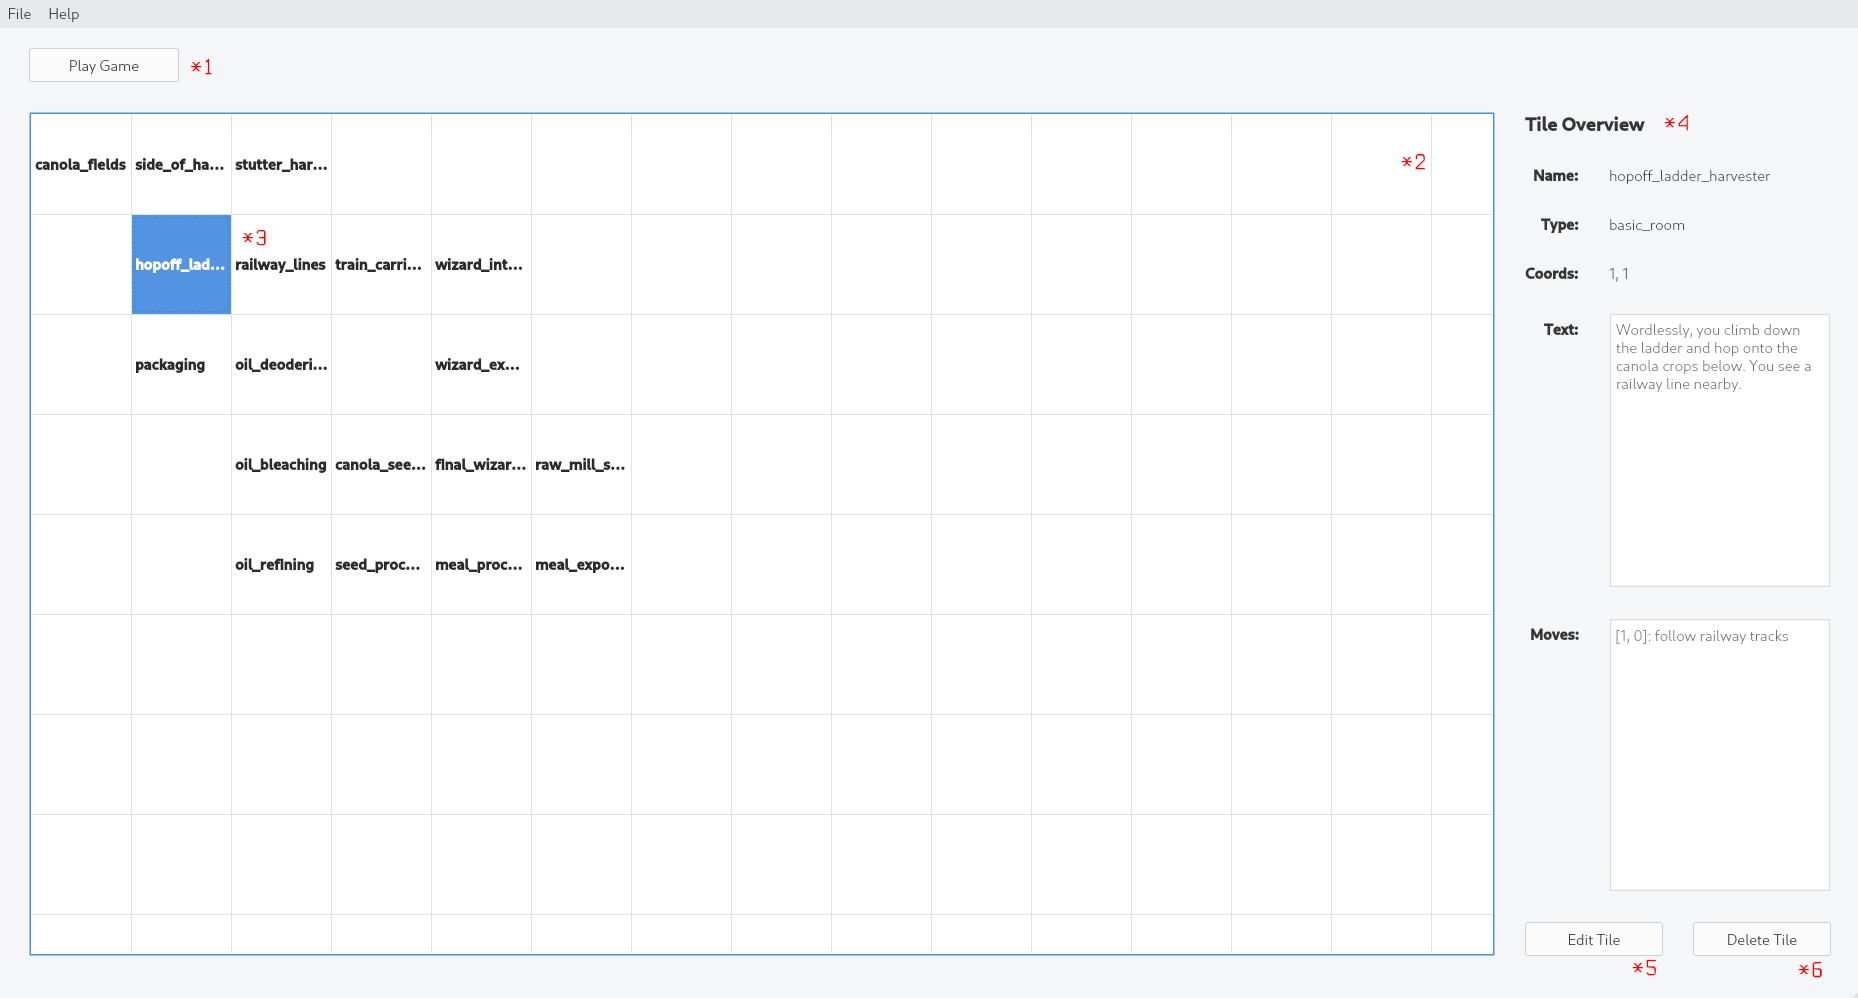
\includegraphics[width=1.0\textwidth]{./mainMenuForm.png}
\end{figure}
This is the main form of \texttt{tbrpggepp}. The elements in this screenshot are labelled as follows:
\begin{enumerate}
	\item "Play Game" button. This opens a terminal in a new window running the text-based game, allowing you to play out your narrative.
	\item The game-world grid. This grid essentially provides a top-down view of the "world" for your text-based game, consisting of hundreds of invisible, empty "tiles" which you may edit and populate with data for the player to interact with. Within this screenshot we see many tiles have already been created and populated with data, thus creating a short text-based adventure. \textbf{Note that at the beginning of every game the player always starts at the topmost leftmost tile, which has coordinates of 0,0.}
	\item You may click on a populated or empty tile to interact with it or view its contents. In this screenshot we see a populated tile has been selected, displaying its contents in the sidebar and allowing the user to either edit it or delelete it by clicking the appropriate buttons.
	\item The sidebar ie. Tile Overview. This presents a read-only view of the contents of the selected tile, including the following elements:
		\begin{itemize}
			\item Name: the unique identifier for a tile, unseen by the player but cannot be reused.
			\item Type: the category of tile, which defines how the user interacts with it. Categories include \texttt{basic\_room} (simply displays text), \texttt{enemy\_room} (contains an enemy for the player to fight), \texttt{item\_room} (contains an item that the player picks up), and \texttt{victory\_room} (identical to a basic tile, except the game ends after the player enters it).
			\item Coords: the X and Y coordinate values of the tile (in that order), representing the tile's location within the game-world.
			\item Text: the words that the player sees upon entering a tile of any type for the first time.
			\item Moves: an overview of the methods in which the player can navigate out of the selected tile. Displays a "coordinate delta" and "label" for each move. The label is simply what the player enters to conduct the move. The "coordinate delta" mathematically represents the change in coordinates applied to the player after conducting the move. For example, a player residing in coordinates 1,1 with a move of [1,0] applied to them would end up in 2,1; which is one unit to the right on the game-world grid. For another example, applying the move [0,-1] on a player residing in 2,6 would move them to 2,5; which is one unit upwards on the game-world grid.
		\end{itemize}
	\item "Edit Tile" button. Clicking this opens the Edit Tile form, allowing you to edit the contents of the currently selected tile. If an empty tile was initially selected then a new tile will be created at its coordinates.
	\item "Delete Tile" button. Clicking this will turn the currently selected tile into an empty tile, handle with care!
	\item An additional element is the "file" menu option in the upper left: this allows you to re-open the Introduction form and open/create a different world file. The "help" option simply links to relevant pages of this document.
\end{enumerate}
\subsubsection{Playing the Game}
As stated above, clicking the "Play Game" button in the Main Menu form will open a terminal in a new window that is running the text-based game. A screenshot of one such terminal is provided below:
\begin{figure}[H]
	\centering
	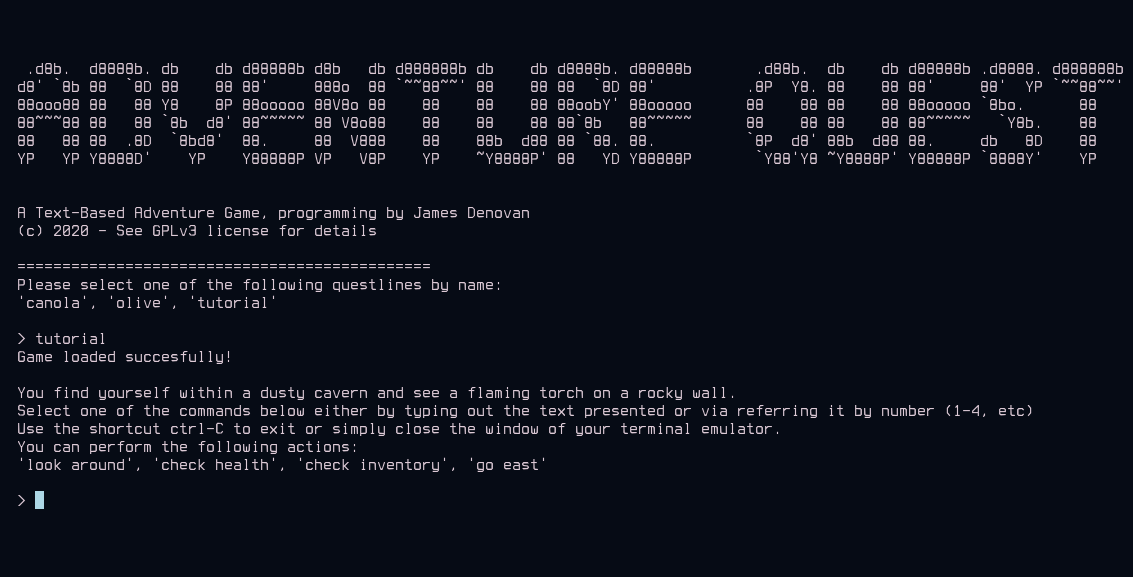
\includegraphics[width=1.0\textwidth]{./gameplay.png}
\end{figure}
When the game program begins, it gives you the decision to choose any of the other game-world files within the directory of your tbrpggepp world file. After loading the desired game-world file, we see the player met with the introductory text of the tile at coordinates0,0; followed by a prompt where the player may either:
\begin{itemize}
	\item Look around: displaying the text in the "Description" field shown in section 2.3
	\item Check health: displaying the current HP value of the player
	\item check inventory: displaying the current inventory of the player
	\item "go east": evidently one of the moves created for the tile at coordinates 0,0.
\end{itemize}
Other scenarios display different prompts, such as when one has consumable health items in their inventory or are engaged in a battle with an enemy. This "tutorial" questline is provided alongside \texttt{tbrpggepp}, which you may want to attempt in order to gain familiarity with \texttt{Adventure Quest}'s style of gameplay.
\newpage
\subsection{Edit Tile Form}
\begin{figure}[H]
	\centering
	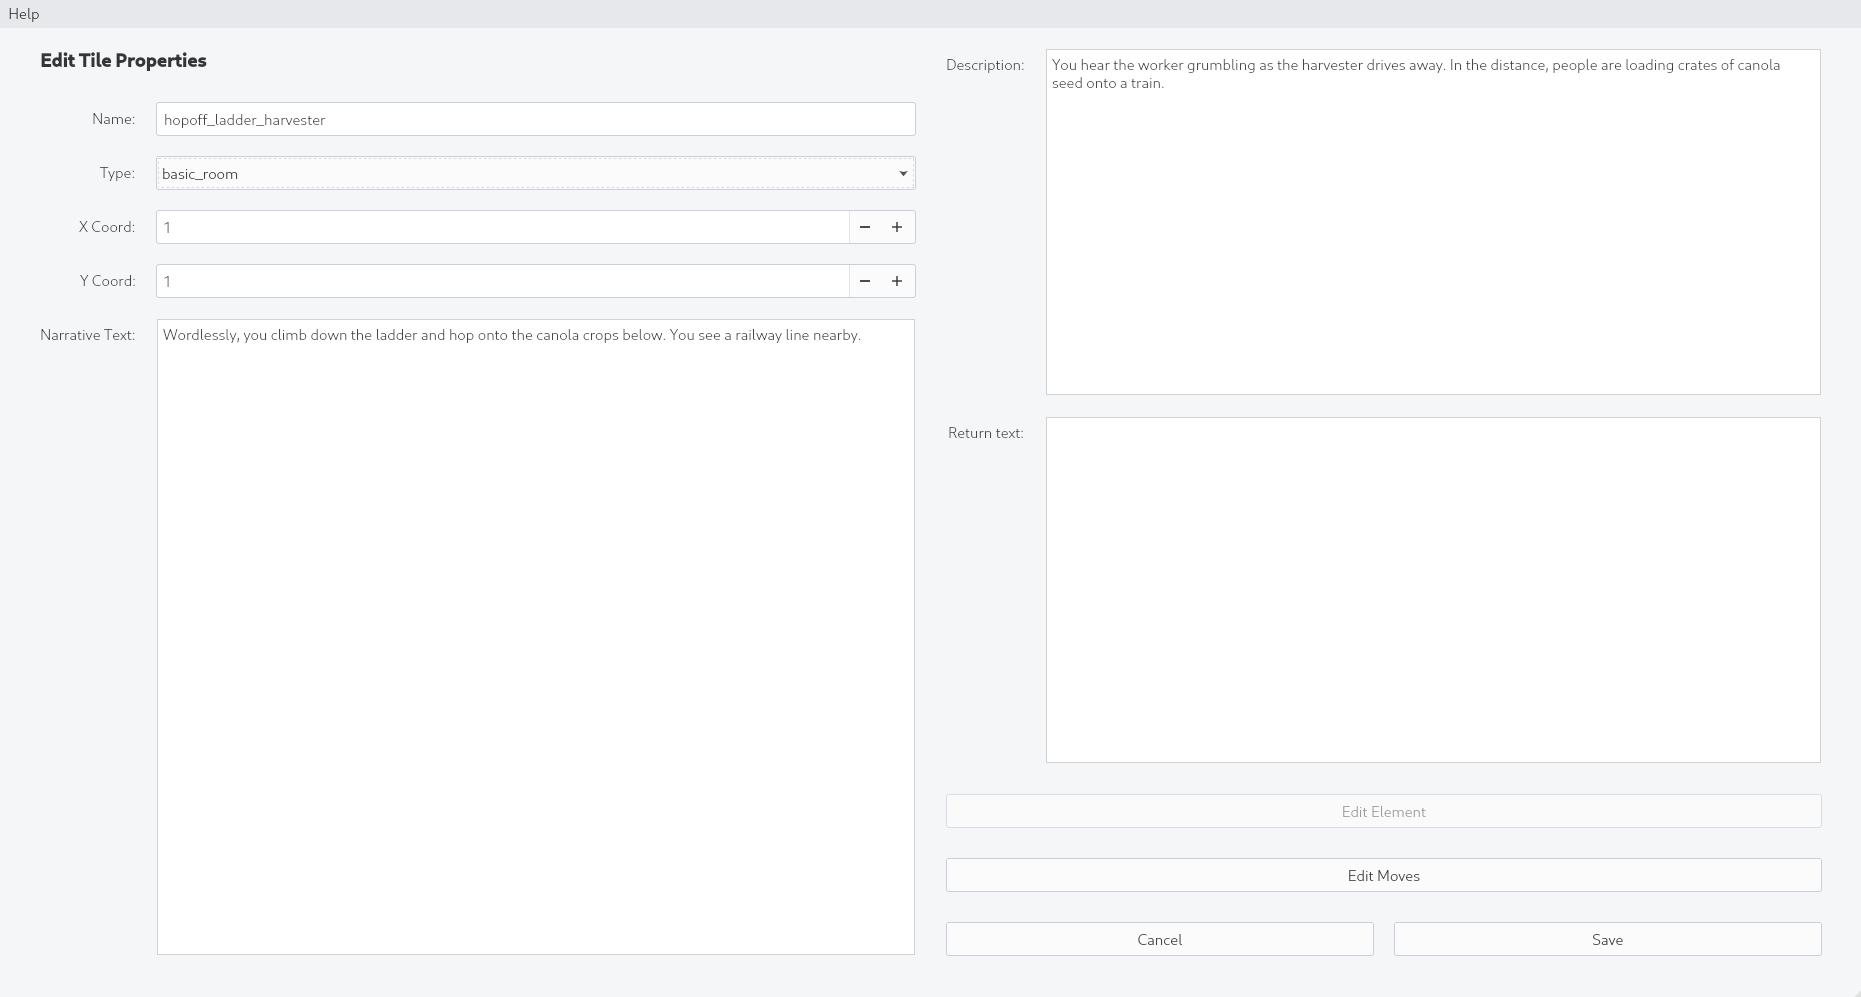
\includegraphics[width=1.0\textwidth]{./editTileFormBasic.png}
\end{figure}
Within this form you can edit the properties of individual tiles. Most of these properties have been described in the previous section, the new properties and UI components are as follows:
\begin{itemize}
	\item Description: the text the player sees when they enter the "\texttt{look around}" action. Should contain a more detailed description of the environment within the tile.
	\item Return Text: the text the player sees when they re-enter the tile after having visited it before. For example, if this were an \texttt{enemy\_room}, the Return Text would contain something like "a defeated enemy lies on the floor".
	\item "Edit Element": This is greyed out because the tile is currently selected to be a "\texttt{basic\_room}" type. Otherwise, this button would either open the Edit item or Edit Enemy form, depending on whether the tile is of type "\texttt{item\_room}" or "\texttt{enemy\_room}" respectively. The text label of the button changes correspondingly as the selected tile type changes as well.
	\item "Edit Moves" button: this opens the Edit Moves form, allowing you to edit the list of moves for the tile.
	\item "Cancel" button: this will close the form and all sub-forms without saving any changed onto the game-map.
	\item "Save" button: this will close the form and all sub-forms while saving all changes in the game-world.
\end{itemize}
\newpage
\subsection{Edit Item Form}
This is the form that is opened when you click the "Edit Item" (otherwise "Edit Element") button within the Edit Tile form, when the tile is of type "\texttt{item\_room}".
\begin{figure}[H]
	\centering
	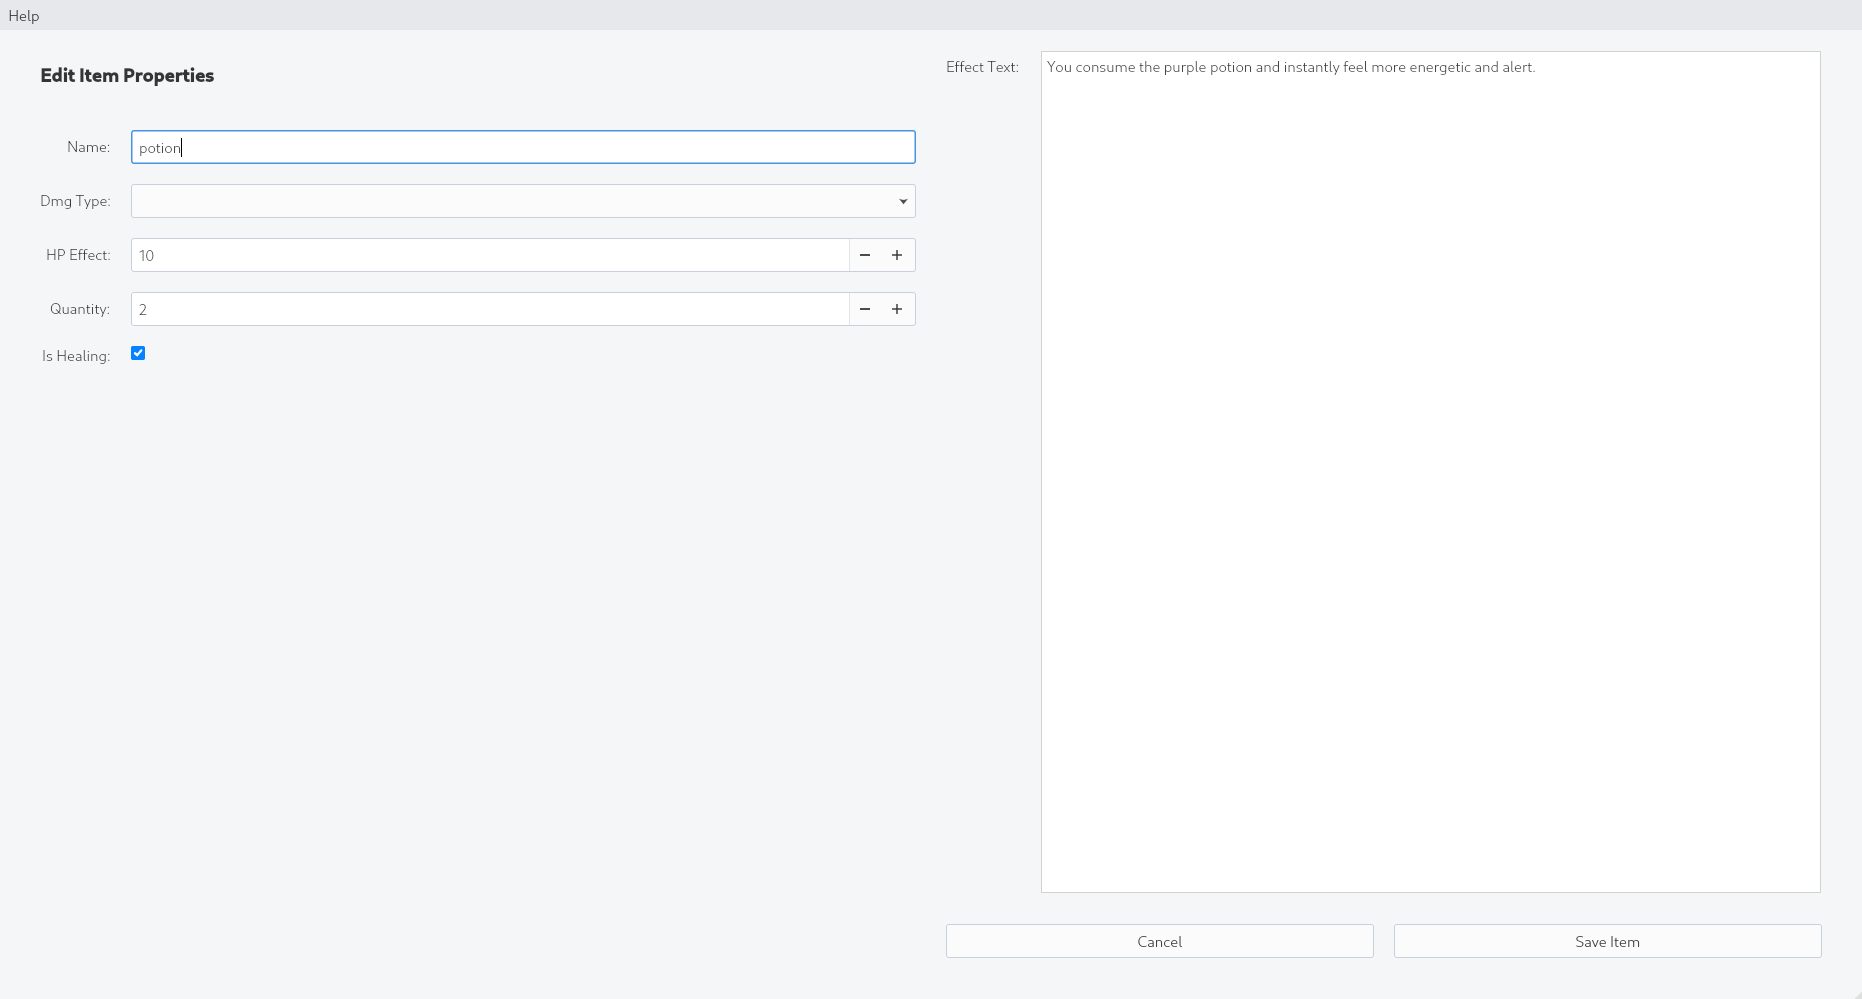
\includegraphics[width=1.0\textwidth]{./editItemForm.png}
\end{figure}
\begin{itemize}
	\item Name: this is the name of the item and will be seen by the player.
	\item Dmg Type: the damage type of the item, in more complicated narratives this feature can be used to enrich gameplay. A weapon of a specific damage type interacting with an enemy of the same damage type deals potentially massive damamge.
	\item HP Effect: the maximum amount of damage inflicted by the item if it is a weapon, or the amount of player health the item heals if it is a consumable healing item. Note that the maximum player HP is 10.
	\item Quantity: the number of items contained in the tile overall. Note that an \texttt{item\_room} tile may only contain one type of item, but may possess multiple items of that type.
	\item "Is Healing" checkbox: Determines whether the item is a weapon inflicting damage, or a consumable healing item.
	\item Effect text: the text displayed to the player after consuming a the item, only relevant if "Is Healing" is checked.
	\item Cancel: closes the form without saving changes.
	\item Save Item: closes the form while saving the item to the parent Edit Tile form.
\end{itemize}

\newpage
\subsection{Edit Enemy Form}
This is the form that is opened when you click the "Edit Enemy" (otherwise "Edit Element") button within the Edit Tile form, when the tile is of type "\texttt{enemy\_room}".
\begin{figure}[H]
	\centering
	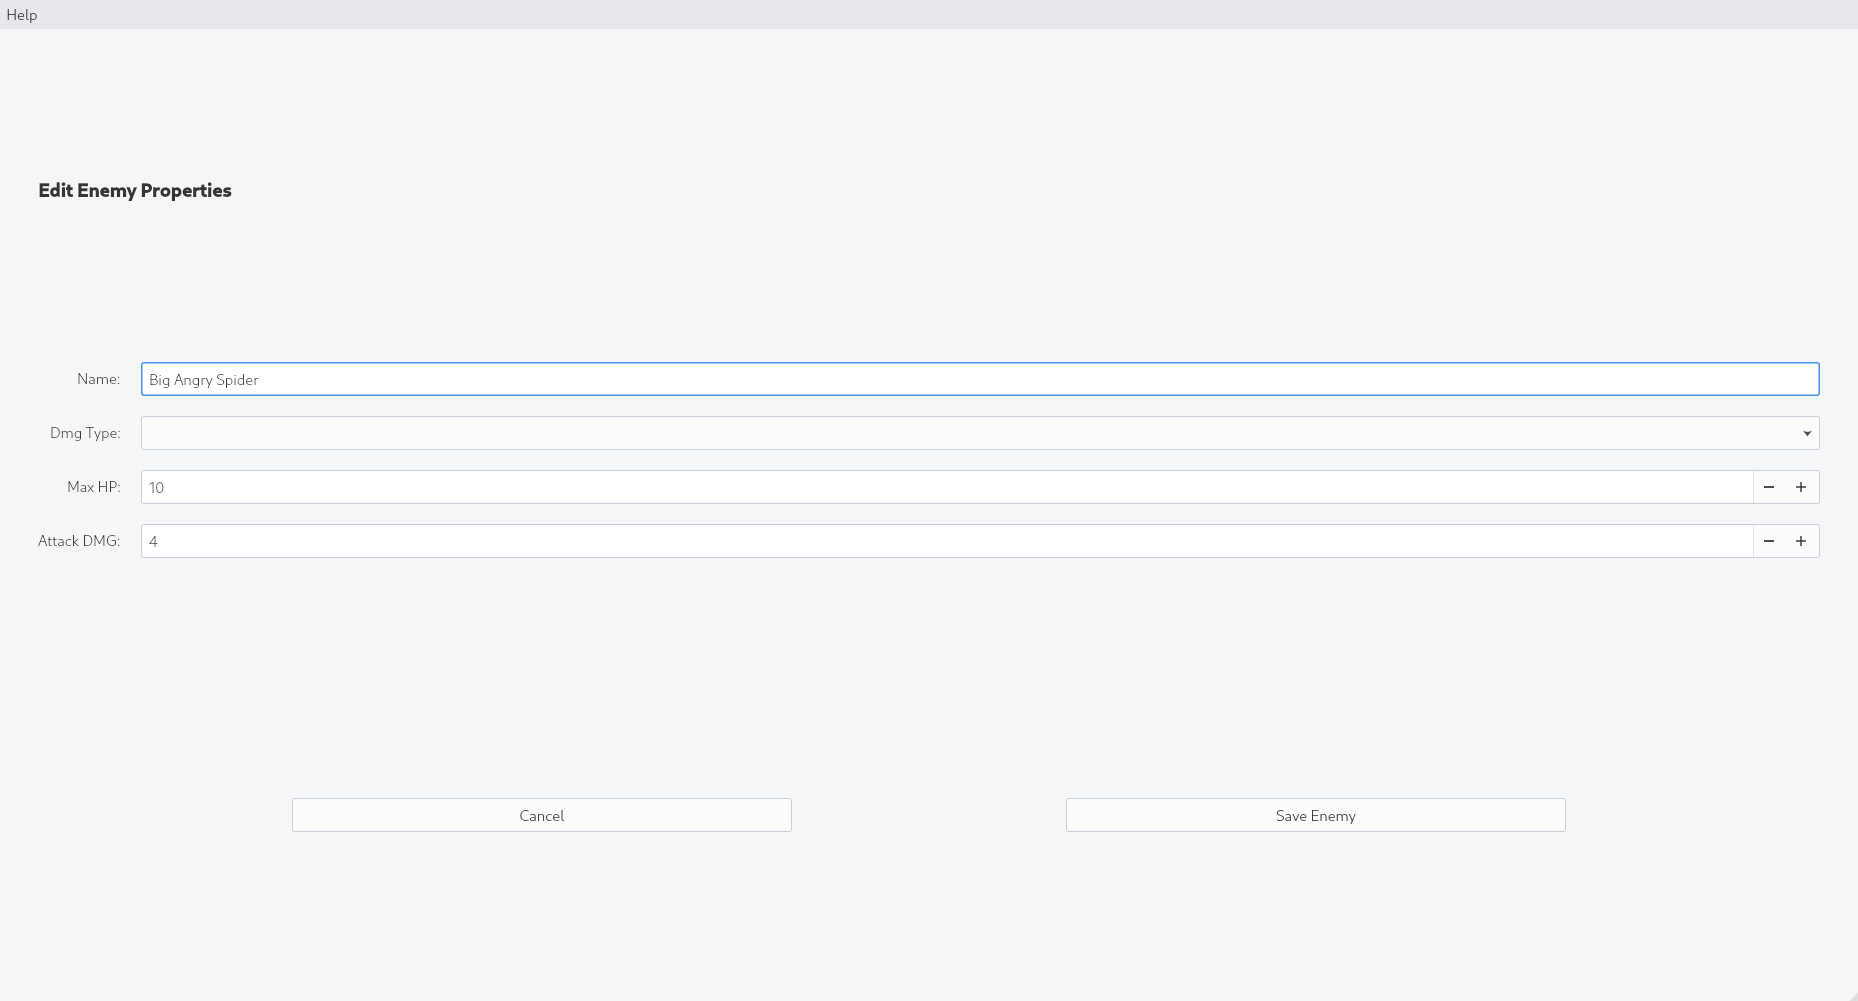
\includegraphics[width=1.0\textwidth]{./editEnemyForm.png}
\end{figure}
\begin{itemize}
	\item Name: this is the name of the enemy and will be seen by the player.
	\item Dmg Type: the damage type of the enemy, in more complicated narratives this feature can be used to enrich gameplay. A weapon of a specific damage type interacting with an enemy of the same damage type deals potentially massive damamge.
	\item Max HP: The maximum number of health points carried by the enemy. Note that the player character starts with maximum health at 10 HP.
	\item Attack Dmg: The maximum number of HP the enemy can detract from the player during one turn of battle.
	\item Cancel: closes the form without saving changes.
	\item Save Item: closes the form while saving the enemy to the parent Edit Tile form.
\end{itemize}
\newpage
\subsection{Edit Moves Form}
This is the form that is opened when you click the "Edit Moves" button within the Edit Tile form.
\begin{figure}[H]
	\centering
	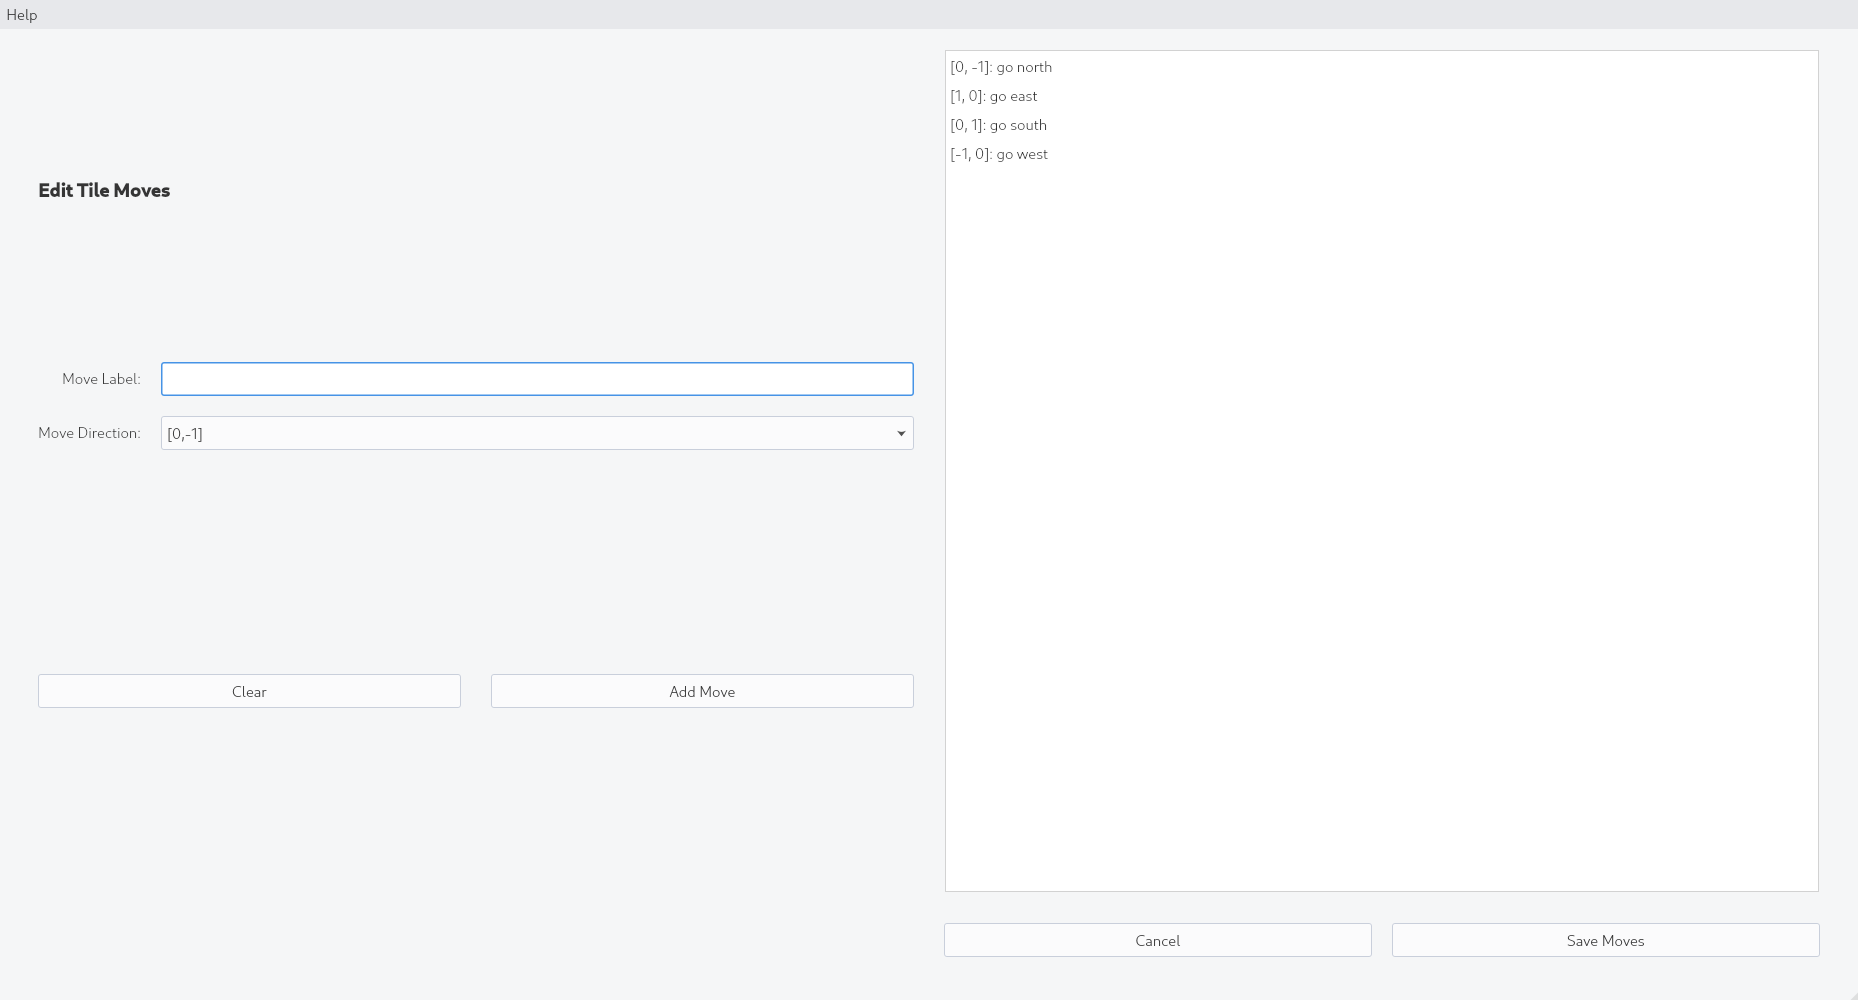
\includegraphics[width=1.0\textwidth]{./editMovesForm.png}
\end{figure}
\begin{itemize}
	\item Move Label: the name of the move, which is visible to the player. The move is executed by the player entering the move label into the game's text prompt.
	\item Move Direction: the "coordinate delta" of the move which as explained in section 2.2, mathematically represents the change in X,Y coordinates which is applied to the player as they execute the move.
	\item "Clear" button: erases the current list of moves for the tile being edited. If this is clicked accidentally, cancel the Edit Moves form and reopen it from the Edit Tile form.
	\item "Add Move" button: adds to the tile's list of moves the new individual move defined by the Label and Direction specified in the above input fields.
	\item On the right-hand side of the form there is a large read-only list box which displays the moves currently assigned to the tile being edited.
	\item Cancel: closes the form without saving changes.
	\item Save Moves: closes the form while saving the updated moves to the parent Edit Tile form.
\end{itemize}
\newpage
\section{Troubleshooting Guide}
\subsection{Issue 1: Invalid world map file!}
\begin{itemize}
	\item This issue is caused simply by not selecting a valid json file. When creating/opening a world-map file, please ensure that the filename ends with "\texttt{.json}".
\end{itemize}
\subsection{Issue 2: No world file selected!}
\begin{itemize}
	\item This issue is caused when one attempts to modify the game-world grid when infact no file has been created or loaded for the Main Menu form. This could have been a result of manually closing the Introduction Form before selecting/creating a file. Please resolve this by using the "file" menu in the top-left of the Main Menu Form to reopen the Introduction form and create/open a valid world-map file.
\end{itemize}
\subsection{Issue 3: Tile name already used!}
\begin{itemize}
	\item Despite the player within the text-game never seeing the given names of tiles, they are essential in that they uniquely define the tile both to the game-designer and the game program internally. Therefore no two tiles can share the same name. \texttt{tbrpggepp} has resolved this temporarily by renaming the newly updated tile with a randomly generated name, which you may rename again to a unique, more human-readable alternative at your leisure.
\end{itemize}
\subsection{Issue 4: Tile name left blank!}
For reasons stated immediately above, the presence of a unique name per each tile is essential to the function of \texttt{tbrpggepp}. Therefore you must enter a unique name into the Edit Tile form before you can save your work.
\subsection{Issue 5: The program crashed!}
Whoops. Please tell me what you were doing immediately before the crash and how you were doing it.
\end{document}
